\section{Auswertung}
\label{sec:Auswertung}






















%\subsection{Untersuchung der Halbwertszeit der beiden Zerfälle bei Silber}
%Die Nullmessung bluzp
%\begin{figure}
%  \centering
%  \includegraphics{Messdaten/silber.pdf}
%  \caption{Zerfallskurve für Silber samt beider Ausgleichgraden zur Bestimmung der verschieden ablaufenden Einzelzerfälle.}
%  \label{fig:silber}
%\end{figure}
%
%\begin{figure}
%  \centering
%  \includegraphics{Messdaten/ergebnis.pdf}
%  \caption{Darstellung des mittels Ausgleichsrechnungen ermittelten summierten Zerfalls sowie der im Experiment gemessenen Werte.}
%  \label{fig:ergebnis}
%\end{figure}
%
%
%

%Bild
%\begin{figure}
%  \centering
%  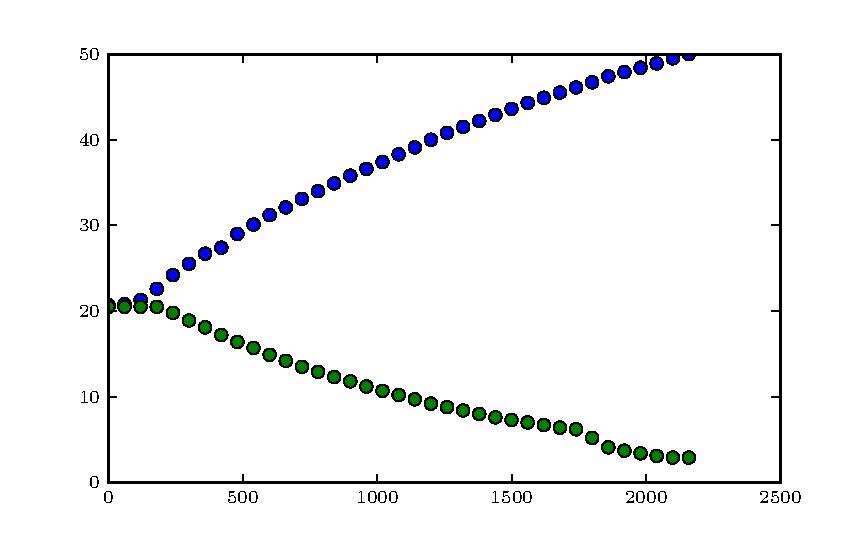
\includegraphics{plot.pdf}
%  \caption{Plot.}
%  \label{fig:plot}
%\end{figure}


%Tabelle
%\begin{table}
%	\centering
%	\caption{Table.}
%	\label{tab:table}
%	\begin{tabular}{ccc}
%		\toprule
%    column1&column2&column3\\
%		\midrule
%		220 & -391 & 659 \\
%		330 & -598 & 946 \\
%		525 & -1000 & 1660 \\
%		702 & -1337 & 2051 \\
%		930 & -1650 & 2450 \\
%		\bottomrule
%	\end{tabular}
%\end{table}
